\documentclass[a4paper,12pt]{article}

% Paquetes básicos
\usepackage[utf8]{inputenc}
\usepackage[T1]{fontenc}
\usepackage[spanish]{babel}
\usepackage{graphicx}
\usepackage{xcolor}
\usepackage{lipsum}
\usepackage{geometry}
\geometry{top=3cm, bottom=3cm, left=2.5cm, right=2.5cm}

% Paquetes para diseño
\usepackage{titlesec}
\usepackage{fancyhdr}
\usepackage{amsmath}
\usepackage{textgreek}
\usepackage{amssymb}
\usepackage{hyperref}

% Paquetes para el entorno lstlisting
\usepackage{listings}
\usepackage{inconsolata}

%encabezado y pie de página nivel profesional
\usepackage{fancyhdr}
\pagestyle{fancy}
\fancyhf{}
\fancyhead[L]{\leftmark}
\fancyhead[R]{\rightmark}
\fancyfoot[L]{\textbf{Ismael Sallami Moreno - GIIADE}}
\fancyfoot[C]{\thepage}
\fancyfoot[R]{\textbf{(UGR)} \today}
\renewcommand{\headrulewidth}{0.4pt}
\renewcommand{\footrulewidth}{0.4pt}
\setlength{\headheight}{15pt}
\setlength{\headsep}{10pt}
\setlength{\footskip}{20pt}
\usepackage{truncate}
\fancyhead[L]{\truncate{0.5\headwidth}{\leftmark}}
\fancyhead[R]{\truncate{0.5\headwidth}{\rightmark}}
\usepackage{mathpazo}
\usepackage{tcolorbox}


% Paquete para fondo
\usepackage{background}
\usepackage{float}

% Configuración de lstlisting
\lstset{
    inputencoding=utf8,          % Permite UTF-8
    extendedchars=true,          % Reconoce caracteres extendidos
    literate=                    % Configuración manual para tildes y símbolos
        {á}{{\'a}}1
        {é}{{\'e}}1
        {í}{{\'i}}1
        {ó}{{\'o}}1
        {ú}{{\'u}}1
        {ñ}{{\~n}}1
        {Á}{{\'A}}1
        {É}{{\'E}}1
        {Í}{{\'I}}1
        {Ó}{{\'O}}1
        {Ú}{{\'U}}1
        {Ñ}{{\~N}}1
        {¿}{{\textquestiondown}}1
        {¡}{{\textexclamdown}}1,
    basicstyle=\ttfamily,        % Fuente monoespaciada
    breaklines=true,             % Habilita salto de línea automático
    frame=single,                % Marco alrededor del código
    backgroundcolor=\color{gray!10}, % Fondo gris claro
    keywordstyle=\color{blue},   % Color para palabras clave
    commentstyle=\color{green},  % Color para comentarios
    stringstyle=\color{red}      % Color para strings
}
\lstdefinestyle{customcpp}{
    language=C++,                % Lenguaje de programación
    showspaces=false,            % No mostrar espacios
    showtabs=false,              % No mostrar tabulaciones
    tabsize=4,                   % Tamaño de tabulación
    showstringspaces=false,      % No mostrar espacios en strings
    numbers=left,                % Números de línea a la izquierda
    numberstyle=\tiny\color{gray}, % Estilo de los números de línea
    numbersep=5pt,               % Separación de los números de línea
    stepnumber=1,                % Mostrar número en cada línea
    basicstyle=\ttfamily\footnotesize, % Estilo básico del código
    keywordstyle=\bfseries\color{blue}, % Estilo de las palabras clave
    commentstyle=\itshape\color{green!50!black}, % Estilo de los comentarios
    stringstyle=\color{red},     % Estilo de los strings
    identifierstyle=\color{black}, % Estilo de los identificadores
    % procnamekeys={def,class},    % Palabras clave para nombres de funciones
    morekeywords={constexpr,nullptr,size_t}, % Más palabras clave
    emph={int,char,double,float,unsigned}, % Palabras a enfatizar
    emphstyle=\color{magenta},   % Estilo de las palabras enfatizadas
    backgroundcolor=\color{gray!10}, % Color de fondo
    frame=shadowbox,             % Marco con sombra
    rulesepcolor=\color{gray},   % Color de la línea de separación
    breakatwhitespace=false,     % No cortar en espacios en blanco
    breaklines=true,             % Cortar líneas largas
    captionpos=b,                % Posición del título (abajo)
    escapeinside={(*@}{@*)},     % Delimitadores para escapar a LaTeX
    morecomment=[l][\color{magenta}]{\#}, % Comentarios de una línea
    morecomment=[s][\color{orange}]{/*}{*/}, % Comentarios multilínea
    morestring=[b],             % Strings entre comillas dobles
    morestring=[b]'              % Strings entre comillas simples
}

% Configuración de título
\titleformat{\section}{\normalfont\Large\bfseries}{\thesection}{1em}{}

% Información del documento
\title{
    \vspace{-2cm}
    
\includegraphics[width=0.3\textwidth]{images/etsiit.png} \\ % Cambia el logo si es necesario
    \LARGE Ingeniería Informática + ADE\\
    \large Universidad de Granada (UGR)\\[1cm]
}
\author{\textbf{Autor:} Ismael Sallami Moreno}
\date{\textbf{Asignatura:} Tema 3: Capa de transporte (FR)\\[1cm]}

% Configuración del fondo
\backgroundsetup{
    scale=1,
    color=black,
    opacity=0.2,
    angle=0,
    position=current page.south,
    vshift=0pt,
    hshift=0pt,
    contents={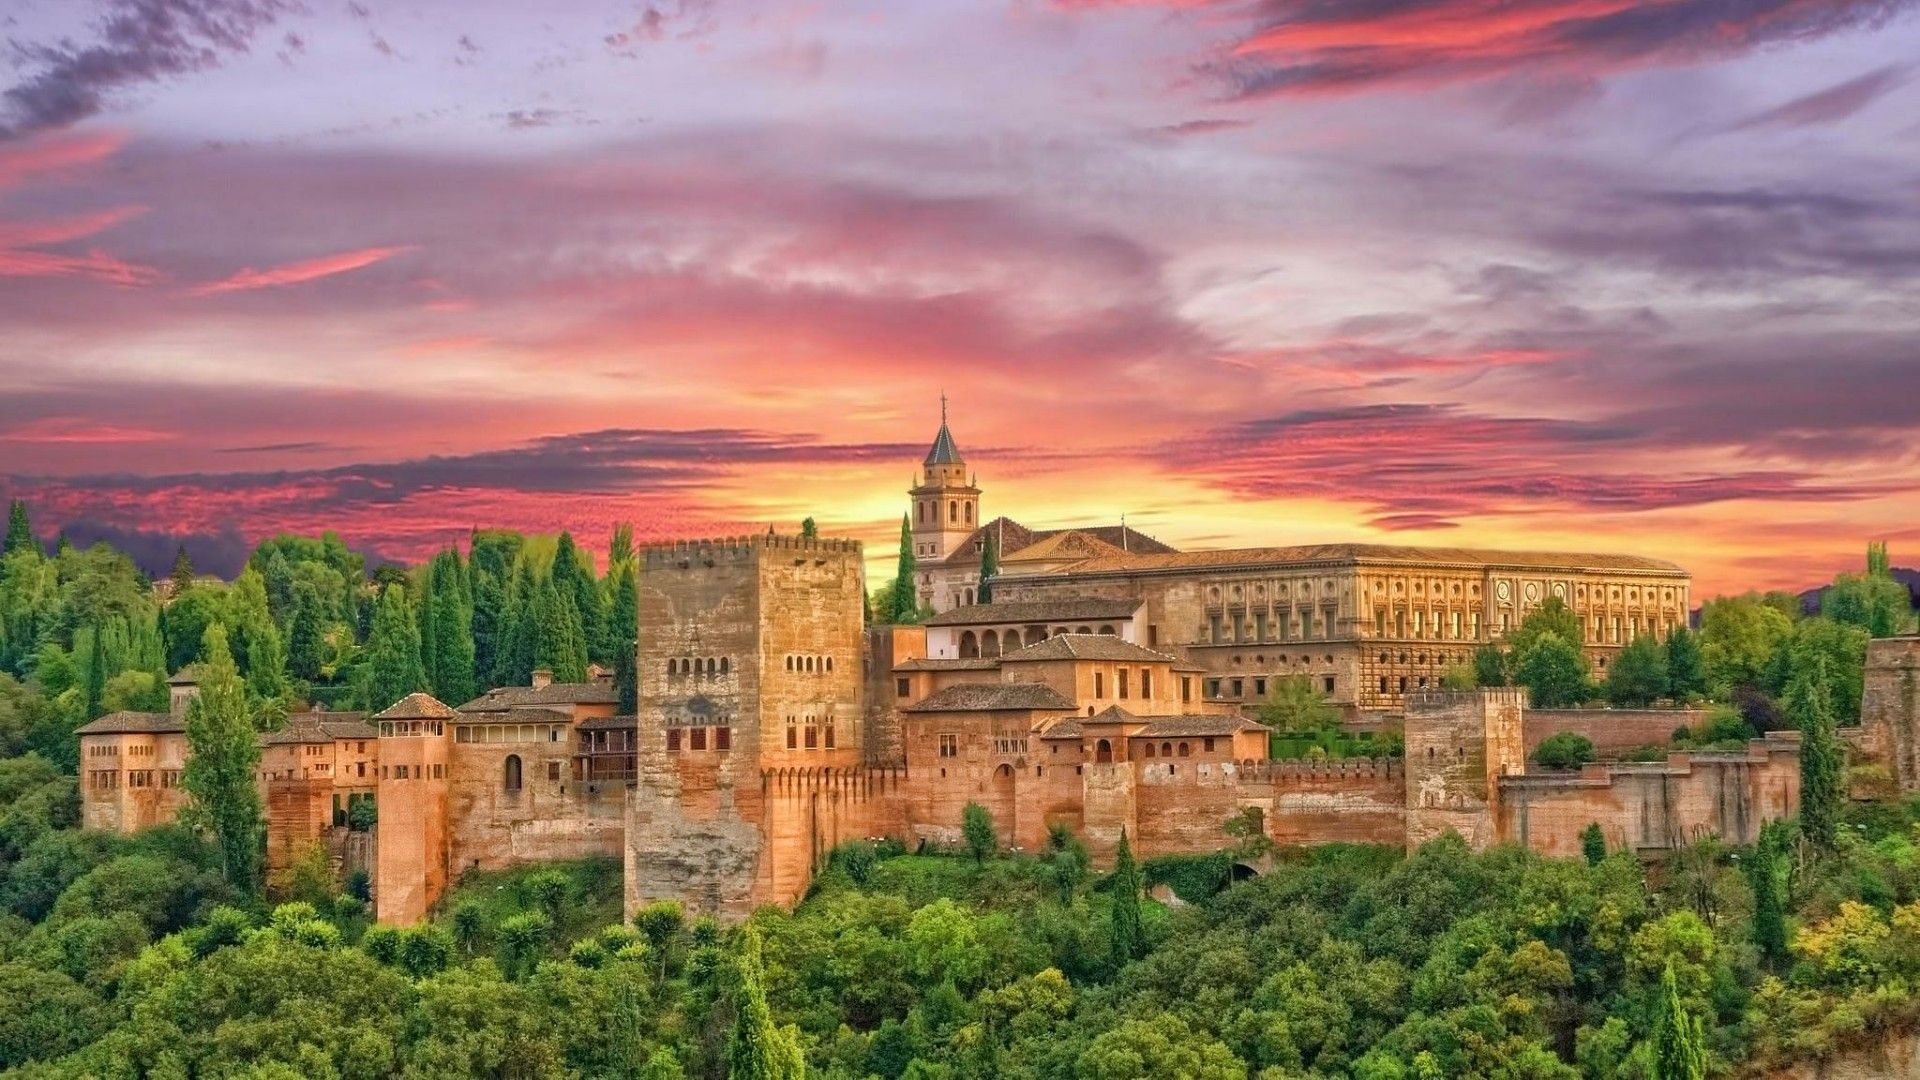
\includegraphics[width=\paperwidth,height=\paperheight,keepaspectratio]{images/granada.jpg}}
}

% Inicio del documento
\begin{document}

% Portada
\maketitle
\thispagestyle{empty}

\begin{center}
    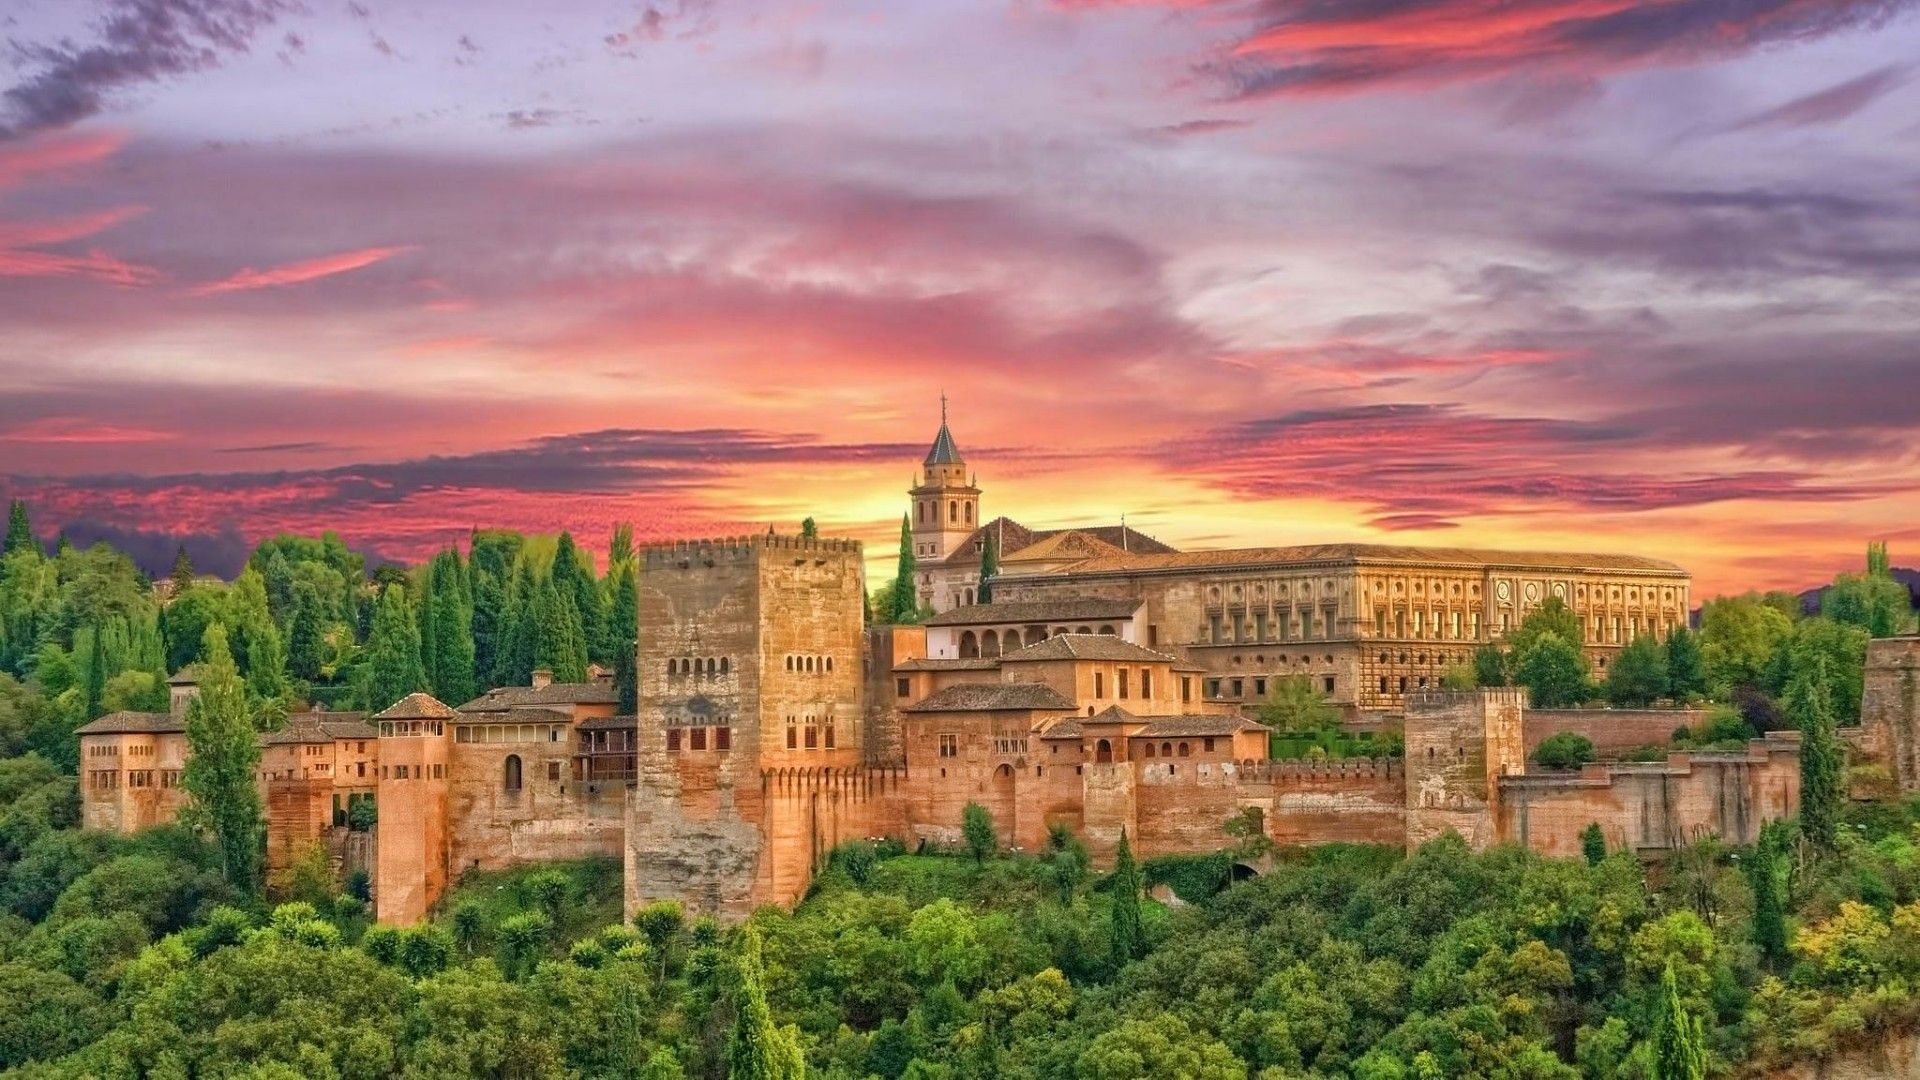
\includegraphics[width=\textwidth,height=0.4\textheight,keepaspectratio]{images/granada.jpg} \\ % Añade tu imagen de fondo
    \vfill
\end{center}

\newpage

% Índice (opcional)
\tableofcontents
\newpage


\section{Introducción}

La capa de transporte es fundamental en el modelo de comunicaciones, proporcionando servicios que garantizan una comunicación efectiva y eficiente entre aplicaciones que se ejecutan en hosts finales. Sus funciones y servicios principales incluyen:

\begin{itemize}
    \item \textbf{Comunicación extremo a extremo (end-to-end):} Garantiza la transmisión de datos entre procesos de aplicación situados en dispositivos distintos a través de una red compleja.
    \item \textbf{Multiplexación y demultiplexación de aplicaciones:} Utiliza puertos para asociar los datos con las aplicaciones correctas.
\end{itemize}

\subsection*{La capa de transporte incluye dos protocolos fundamentales:
}
\subsection*{Protocolo de datagrama de usuario (UDP)}
\begin{itemize}
    \item Permite la multiplexación y demultiplexación de aplicaciones\footnote{En el contexto de la capa de transporte, la multiplexación se refiere al proceso mediante el cual múltiples flujos de datos de diferentes aplicaciones o procesos dentro de un host se combinan para ser transmitidos a través de una única conexión de red. Esto se realiza asignando identificadores únicos, como números de puerto, a cada flujo de datos, lo que permite a la capa de transporte diferenciarlos y enviarlos correctamente al destinatario correspondiente.

    La demultiplexación es el proceso inverso: cuando los datos llegan al host receptor, la capa de transporte utiliza esos identificadores (puertos) para separar los flujos de datos y entregarlos a las aplicaciones o procesos adecuados. Esto asegura que la información llegue al lugar correcto, incluso si varios procesos están utilizando la red simultáneamente.}
    \item Proporciona un servicio no orientado a conexión, caracterizado por su simplicidad y ausencia de confiabilidad.
\end{itemize}

\subsection*{Protocolo de control de transmisión (TCP)}
\begin{itemize}
    \item Permite la multiplexación y demultiplexación de aplicaciones.
    \item Ofrece un servicio orientado a conexión y confiable, destacándose por:
    \begin{itemize}
        \item Control de errores y de flujo.
        \item Gestión de la conexión (establecimiento y cierre).
        \item Control de congestión para optimizar el uso de la red.
    \end{itemize}
\end{itemize}

Además, TCP ha evolucionado con extensiones que se adaptan a las necesidades de redes modernas, manteniendo la interoperabilidad entre los extremos y mejorando su rendimiento en diversos escenarios.

\subsection{Comunicación Extremo a Extremo}

La comunicación extremo a extremo en la capa de transporte asegura que los datos se transfieran directamente entre las aplicaciones en los hosts emisores y receptores. Este modelo se ilustra en el diagrama mostrado en la página 7 del material, que detalla la interacción entre las capas de aplicación, transporte y red:

\begin{figure}[H]
    \centering
    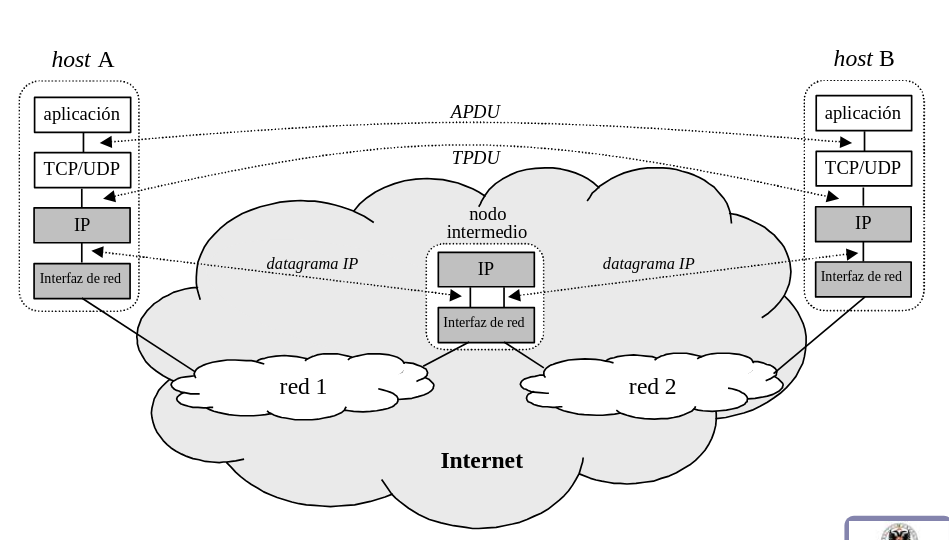
\includegraphics[width=0.9\textwidth]{images/end-to-end.png}
    \caption{Esquema de comunicación extremo a extremo.}
    \label{fig:end_to_end}
\end{figure}

En el esquema, se destacan los siguientes elementos clave:
\begin{itemize}
    \item \textbf{Capas de red y transporte:} Cada host (A y B) utiliza estas capas para encapsular y enviar los datos hacia la aplicación correspondiente en el otro extremo.
    \item \textbf{Datagramas IP y TPDU:} Los datagramas IP son utilizados por la capa de red para transportar las Unidades de Datos del Protocolo de Transporte (TPDU) entre los hosts.
    \item \textbf{APDU (Application Protocol Data Unit):} 
        \begin{itemize}
            \item Las APDU son las unidades de datos utilizadas en la capa de aplicación para la comunicación entre aplicaciones en diferentes sistemas.
            \item En el contexto de la capa de transporte, las APDU se encapsulan en segmentos TCP o datagramas UDP, dependiendo del protocolo utilizado.
            \item La capa de transporte se encarga de la multiplexación y demultiplexación de estas APDU, asegurando que se entreguen a la aplicación correcta en el host de destino.
            \item Las APDU contienen la información específica de la aplicación, como comandos, respuestas y datos de usuario, que se transmiten de manera confiable (TCP) o no confiable (UDP) a través de la red.
        \end{itemize}
    \item \textbf{Intermediarios:} Los nodos intermedios en la red solo manejan el nivel de red, garantizando la entrega de los datagramas IP sin interactuar con las capas superiores.
    \item \textbf{Capas de aplicación:} Las aplicaciones en ambos extremos envían y reciben datos procesados por las capas inferiores, asegurando la comunicación.
\end{itemize}

Este enfoque modular permite la interoperabilidad y confiabilidad en redes complejas, separando claramente las responsabilidades entre las distintas capas.

\section{Protocola de Datagrama del Usuario (UDP)}

Las siglas significan User Datagram Protocol, se trata de un protocolo que se basa en la funcionalidad de \textbf{best effor}.
Se trata de un servicio que lleva a cabo el transporte entre redes, es no orientado a conexión, no handshaking\footnote{El \textit{handshaking} es un proceso de comunicación entre dos dispositivos que establece las reglas para la transmisión de datos. Este proceso asegura que ambos dispositivos estén sincronizados y listos para intercambiar información.}, además no hay retardos en el establecimiento y cada TPDU\footnote{TPDU significa \textit{Transport Protocol Data Unit} (Unidad de Datos del Protocolo de Transporte). Es la unidad de datos que se intercambia entre entidades de la capa de transporte en un modelo de red, como el modelo OSI.} es independiente.\\\\
Además, abarca las características de multiplexación y demultiplexación, las cuales ayudan a transportar las TPDU al proceso correcto.\\\\
Existen algunos puertos con servicios normalizados, como es el caso del puerto 7 que es un \textit{echo} con función Eco, el 13 que es \textit{daytime} con función fecha, etc. Por otro lado, hay otros puertos que están libres para el uso propio del desarrollador.\\\\
\begin{table}[H]
    \centering
    \begin{tabular}{|c|p{5cm}|p{5cm}|}
    \hline
    \textbf{Puerto} & \textbf{Aplicación/Servicio} & \textbf{Descripción} \\ \hline
    7 & echo & Eco \\ \hline
    13 & daytime & Fecha \\ \hline
    37 & time & Hora \\ \hline
    42 & nameserver & Servicio de nombres \\ \hline
    53 & domain & Servicio de nombres de dominio \\ \hline
    69 & tftp & Transferencia simple de ficheros \\ \hline
    123 & ntp & Protocolo de tiempo de red \\ \hline
    \end{tabular}
\end{table}
UDP se suele usar para servicios multimedia, debido a que es tolerante a fallos y sensible frente a los retardos que se puedan producir.\\\\
Cada segmento UDP se encapsula en un datagrama IP. Esto significa que el segmento UDP, que contiene los datos de la aplicación y los encabezados UDP, se coloca dentro de la carga útil de un datagrama IP. El datagrama IP, a su vez, añade su propio encabezado, que incluye información necesaria para el enrutamiento y la entrega a través de la red IP. De esta manera, los datos de la aplicación pueden ser transmitidos de manera eficiente a través de la red.

\section{Protocolo de Control de Transmisión (TCP)}

\subsection*{Características del Transmission Control Protocol (TCP)}

El protocolo TCP, definido en diversos RFCs (793, 1122, 1323, 2018, 2581), ofrece un conjunto de características que lo hacen adecuado para la transmisión fiable de datos en redes complejas. Estas características incluyen:

\begin{itemize}
    \item \textbf{Servicio punto a punto:} TCP establece una conexión directa entre dos hosts, permitiendo una comunicación exclusiva entre ellos.
    \item \textbf{Servicio orientado a conexión:} Requiere un estado común entre el emisor y el receptor, logrado a través de un procedimiento de inicialización denominado \textit{hand-shaking}.
    \item \textbf{Entrega ordenada:} Asegura que las secuencias de bytes generadas por la aplicación lleguen en el orden correcto al receptor, proporcionando un servicio \textit{stream oriented}.
    \item \textbf{Transmisión full-duplex:} Permite la transmisión simultánea de datos en ambas direcciones entre los hosts.
    \item \textbf{Mecanismo de detección y recuperación de errores:} Emplea esquemas ARQ (\textit{Automatic Repeat reQuest}) con confirmaciones positivas acumulativas (ACKs) y temporizadores adaptables (\textit{timeouts}).
    \item \textbf{Control de congestión y flujo:} Utiliza ventanas deslizantes de tamaño máximo adaptable para garantizar un uso eficiente de los recursos de red y evitar saturaciones.
    \item \textbf{Incorporación de confirmaciones (\textit{piggybacking}):} Los ACKs pueden ser integrados en segmentos de datos para optimizar el uso del ancho de banda.
\end{itemize}


En cuanto a las funcionalidades de TCP encontramos las siguientes: multiplexación y demultiplexación de aplicaciones, control de la conexión (establecimiento y cierre), control de errores y flujo y el control de la gestión.

\begin{figure}[H]
    \centering
    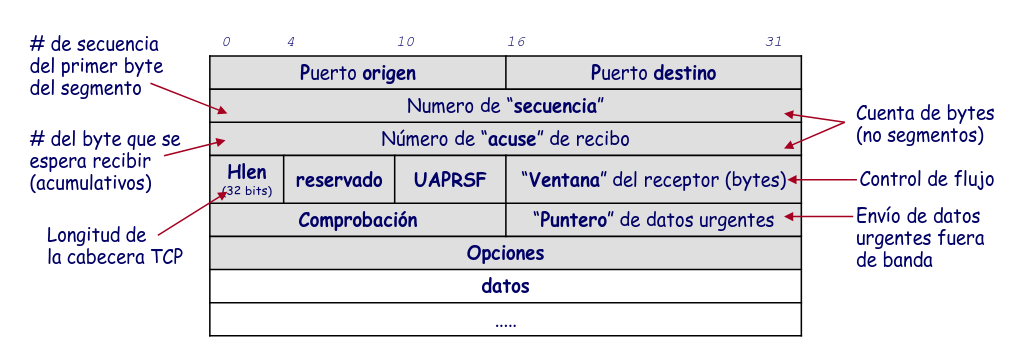
\includegraphics[width=0.9\textwidth]{images/tpdu.png}
    \caption{Estructura de un segmento TCP.}
    \label{fig:tcp}
\end{figure}

\subsection{Multliplexación y Demultiplexación}

Sirven para transportar las TPDU al proceso correcto, hay una serie de puertos asignados por defecto con servicio:
\begin{table}[H]
    \centering
    \begin{tabular}{|c|p{5cm}|p{5cm}|}
    \hline
    \textbf{Puerto} & \textbf{Aplicación/Servicio} & \textbf{Descripción} \\ \hline
    20 & FTP-DATA & Transferencia de ficheros: datos \\ \hline
    21 & FTP & Transferencia de ficheros: control \\ \hline
    22 & SSH & Terminal seguro \\ \hline
    23 & TELNET & Acceso remoto \\ \hline
    25 & SMTP & Correo electrónico \\ \hline
    53 & DNS & Servicio de nombres de dominio \\ \hline
    80 & HTTP & Acceso hipertexto (web) \\ \hline
    110 & POP3 & Descarga de correo \\ \hline
    \end{tabular}
\end{table}



Al igual que en anterior caso, hay otros puertos libres.\\\\
La conexión TCP se identifica por le puerto e IP tanto de origen como de destino.


\subsection{Control de conexión}

TCP ofrece un servicio orientado a conexión. El intercambio de la información tiene 3 fases:
\begin{itemize}
    \item Establecimiento de la conexión: three-way handshake
    \item Intercambio de datos
    \item Cierre de la conexión
\end{itemize}

\subsection*{Three-way Handshake en TCP}

El \textbf{three-way handshake} (o apretón de manos en tres pasos) es un proceso fundamental en el protocolo TCP (Transmission Control Protocol) que permite establecer una conexión confiable entre dos dispositivos (por ejemplo, un cliente y un servidor) antes de comenzar a transmitir datos. Este proceso asegura que ambos dispositivos están listos para la comunicación y pueden manejar los datos de manera adecuada.

El \textbf{three-way handshake} se lleva a cabo en tres pasos:

\begin{enumerate}
    \item \textbf{SYN (Synchronize)}:
    \begin{itemize}
        \item El cliente (el dispositivo que inicia la conexión) envía un segmento TCP con la bandera \textbf{SYN} activada. Este mensaje indica que el cliente desea establecer una conexión y está listo para sincronizar sus secuencias de números.
        \item El mensaje también contiene un número de secuencia inicial que se utilizará para los datos que se transmitirán más adelante.
    \end{itemize}

    \item \textbf{SYN-ACK (Synchronize-Acknowledge)}:
    \begin{itemize}
        \item El servidor, al recibir el paquete SYN del cliente, responde enviando un segmento TCP con las banderas \textbf{SYN} y \textbf{ACK} activadas.
        \item El \textbf{SYN} indica que el servidor acepta la solicitud de conexión y está listo para comunicarse.
        \item El \textbf{ACK} (Acknowledge) confirma la recepción del paquete SYN del cliente y le informa que ha recibido el número de secuencia del cliente. Además, el servidor incluye su propio número de secuencia, que se utilizará para las respuestas.
    \end{itemize}

    \item \textbf{ACK (Acknowledge)}:
    \begin{itemize}
        \item Finalmente, el cliente envía un paquete de confirmación (ACK) al servidor, indicando que ha recibido correctamente el paquete SYN-ACK.
        \item A partir de este momento, la conexión está completamente establecida, y los dos dispositivos pueden comenzar a intercambiar datos.
    \end{itemize}
\end{enumerate}

Este proceso de tres pasos asegura que tanto el cliente como el servidor estén listos para enviar y recibir datos, y que la conexión se realice de manera confiable, manteniendo un control adecuado de las secuencias de los paquetes de datos que se transmitirán.

\textbf{Resumen}:

\begin{enumerate}
    \item \textbf{Cliente $\to$ SYN} (solicita la conexión)
    \item \textbf{Servidor $\to$ SYN-ACK} (responde aceptando la solicitud)
    \item \textbf{Cliente $\to$ ACK} (confirma la conexión)
\end{enumerate}

Este método es una de las razones por las que TCP es considerado un protocolo orientado a la conexión y confiable.


\subsubsection{Números de Secuencia.}

El número de secuencia es un campo de 32 bits que cuenta bytes en módulo $2^{32}$ (el contador se da la vuelta cuando llega al valor máximo). Este número de secuencia no empieza normalmente en 0, sino en un valor denominado \textit{ISN} (Initial Sequence Number), elegido teóricamente al azar, para evitar confusiones con solicitudes anteriores.\\\\

El \textit{ISN} es elegido por el sistema (cliente o servidor). El estándar sugiere utilizar un contador entero incrementado en 1 cada 4 μs aproximadamente. En este caso, el contador se da la vuelta (y el \textit{ISN} reaparece) al cabo de 4 horas y 46 minutos.\\\\
El mecanismo de selección de los \textit{ISN} es suficientemente fiable para proteger de coincidencias, pero no es un mecanismo de protección frente a sabotajes. Es relativamente fácil averiguar el \textit{ISN} de una conexión e interceptarla, suplantando a alguno de los dos participantes.\\\\

TCP incrementa el número de secuencia de cada segmento según los bytes que tenía el segmento anterior, con una sola excepción: cuando los flags \textbf{SYN} o \textbf{FIN} están activados, incrementan en 1 el número de secuencia. La presencia del flag \textbf{ACK} no incrementa el número de secuencia.\\\\

\subsubsection{Establecimiento de Conexión TCP con el Three-Way Handshake}

A continuación, se describen los pasos implicados en este proceso (Caso normal):

\begin{figure}[H]
    \centering
    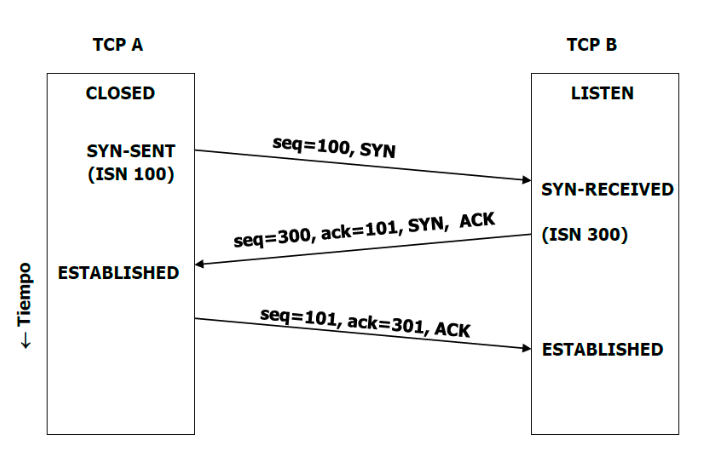
\includegraphics[width=0.7\textwidth]{images/caso_normal.png}
    \caption{Caso Normal en TCP}
    \label{fig:three_way_handshake}
\end{figure}

\begin{itemize}
    \item \textbf{Paso 1: SYN} - TCP A envía un segmento con el flag SYN activado y un número de secuencia inicial (ISN) de 100 a TCP B. Este segmento se representa como \texttt{SYN seq=100}.
    \item \textbf{Paso 2: SYN-ACK} - TCP B responde con un segmento que tiene el flag SYN activado, un ISN de 300, y un número de acuse de recibo (ACK) de 101 (que es el ISN de TCP A más 1). Este segmento se representa como \texttt{SYN-ACK seq=300 ack=101}.
    \item \textbf{Paso 3: ACK} - Finalmente, TCP A envía un segmento con el flag ACK activado, un número de secuencia de 101 (ISN de TCP A más 1), y un número de acuse de recibo de 301 (ISN de TCP B más 1). Este segmento se representa como \texttt{ACK seq=101 ack=301}.
\end{itemize}

Después de estos tres pasos, la conexión TCP se establece y ambos puntos finales pueden comenzar a intercambiar datos de manera fiable. Este proceso es crucial para la comunicación en redes TCP/IP, ya que asegura que ambos puntos finales están preparados para recibir y enviar datos.

\begin{figure}[H]
    \centering
    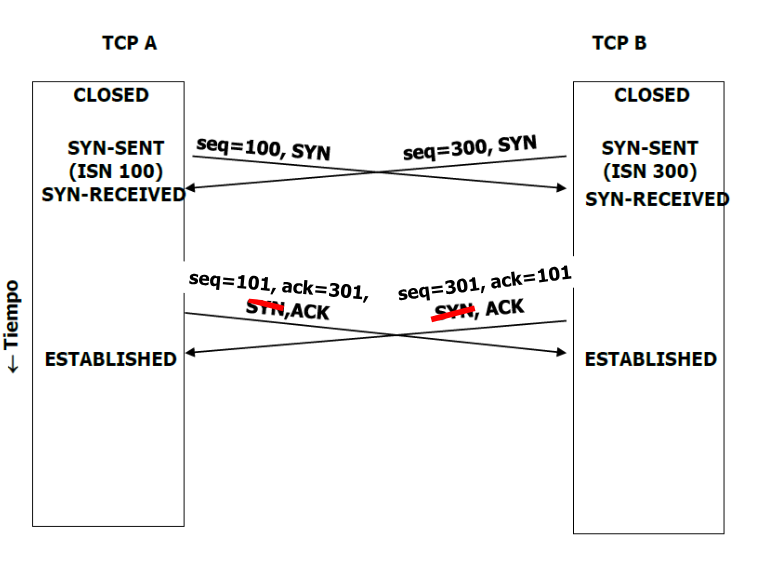
\includegraphics[width=0.7\textwidth]{images/tcp_control_conex.png}
    \caption{Proceso de Three-Way Handshake en TCP}
    \label{fig:three_way_handshake}
\end{figure}

\subsubsection{Establecimiento de la Conexión TCP: Caso con SYN Retrasados y Duplicados}

A continuación se describen los eventos representados en el diagrama :

\begin{itemize}
    \item \textbf{TCP A:}
    \begin{itemize}
        \item \textbf{SYN-SENT (ISN 90):} TCP A envía un segmento SYN con un número de secuencia inicial (ISN) de 90.
        \item \textbf{CLOSED (timeout):} Debido a un tiempo de espera, TCP A cierra la conexión.
        \item \textbf{SYN-SENT (ISN 100):} TCP A vuelve a enviar un segmento SYN, esta vez con un ISN de 100.
        \item \textbf{Paquetes SYN duplicados y retrasados:} Varios segmentos SYN con los ISN 90 y 100 se envían, representando paquetes duplicados y retrasados.
        \item \textbf{Respuesta de TCP B:} TCP B responde con un segmento \texttt{SYN-ACK seq=300 ack=91}, y TCP A envía un segmento \texttt{RST seq=91}.
        \item \textbf{Nuevo intento con ISN 100:} TCP A vuelve a enviar un segmento SYN con ISN 100.
        \item \textbf{SYN-ACK con ISN 400:} TCP B responde con \texttt{SYN-ACK seq=400 ack=101}, y TCP A confirma con un \texttt{ACK seq=101 ack=401}.
        \item \textbf{Conexión establecida:} Finalmente, se establece la conexión y ambos puntos finales entran en el estado \texttt{ESTABLISHED}.
    \end{itemize}

    \item \textbf{TCP B:}
    \begin{itemize}
        \item \textbf{LISTEN:} TCP B espera la llegada de un segmento SYN.
        \item \textbf{SYN-RECEIVED (ISN 300):} TCP B recibe un segmento SYN y responde, entrando en estado \texttt{SYN-RECEIVED}.
        \item \textbf{Recepción de paquetes duplicados:} TCP B recibe varios segmentos SYN con ISN 90 y responde con un \texttt{RST seq=91}.
        \item \textbf{Nuevo SYN-RECEIVED (ISN 400):} TCP B recibe un nuevo SYN con ISN 100, responde con \texttt{SYN-ACK seq=400 ack=101}.
        \item \textbf{Conexión establecida:} Tras recibir el \texttt{ACK seq=101 ack=401} de TCP A, la conexión se establece y ambos puntos finales entran en el estado \texttt{ESTABLISHED}.
    \end{itemize}
\end{itemize}

Esta secuencia demuestra cómo TCP maneja paquetes retrasados y duplicados, asegurando la fiabilidad de la conexión a pesar de las posibles interrupciones y retransmisiones.

\begin{figure}[H]
    \centering
    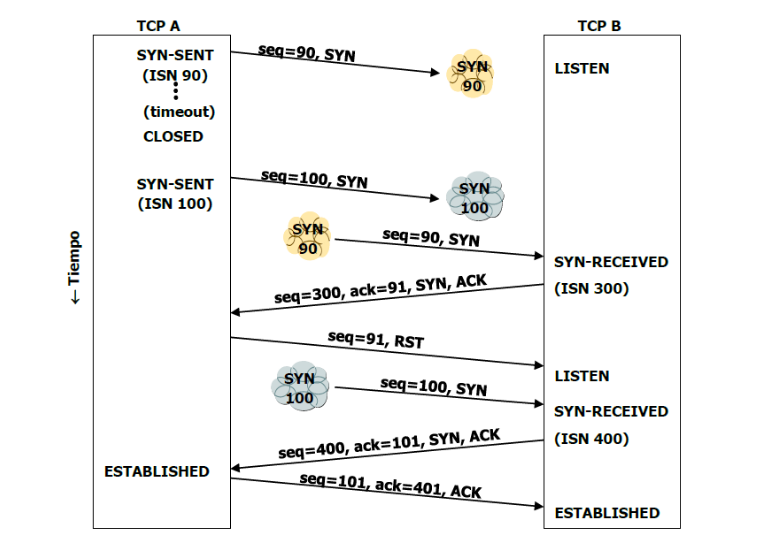
\includegraphics[width=0.7\textwidth]{images/control_conex_retrasado.png}
    \caption{Establecimiento de la Conexión TCP con Paquetes SYN Retrasados y Duplicados}
    \label{fig:tcp_syn_retrasados_duplicados}
\end{figure}

\subsubsection{Establecimiento de la Conexión Simultánea en TCP}

A continuación, se describe el proceso paso a paso (caso raro):

\begin{itemize}
    \item \textbf{Estado inicial:} Ambos puntos, TCP A y TCP B, comienzan en el estado \texttt{CLOSED}.
    \item \textbf{SYN (TCP A):} TCP A envía un segmento SYN con un número de secuencia inicial (ISN) de 100 y pasa al estado \texttt{SYN-SENT}.
    \item \textbf{SYN (TCP B):} Simultáneamente, TCP B envía un segmento SYN con un ISN de 300 y también pasa al estado \texttt{SYN-SENT}.
    \item \textbf{SYN-ACK (Ambos):} Al recibir el SYN del otro punto final, ambos TCP A y TCP B envían un segmento SYN-ACK. TCP A envía \texttt{SYN-ACK seq=101 ack=301}, y TCP B envía \texttt{SYN-ACK seq=301 ack=101}.
    \item \textbf{ACK (Ambos):} Finalmente, ambos puntos finales envían un segmento ACK confirmando la recepción de los segmentos SYN-ACK. TCP A envía \texttt{ACK seq=101 ack=301} y TCP B envía \texttt{ACK seq=301 ack=101}.
    \item \textbf{Estado \texttt{ESTABLISHED}:} La conexión se establece y ambos puntos finales entran en el estado \texttt{ESTABLISHED}, listos para la transferencia de datos.
\end{itemize}

Este proceso de establecimiento simultáneo de conexión es una demostración de la capacidad de TCP para manejar conexiones iniciadas por ambos puntos finales al mismo tiempo, garantizando la sincronización y el control adecuados.

\begin{figure}[H]
    \centering
    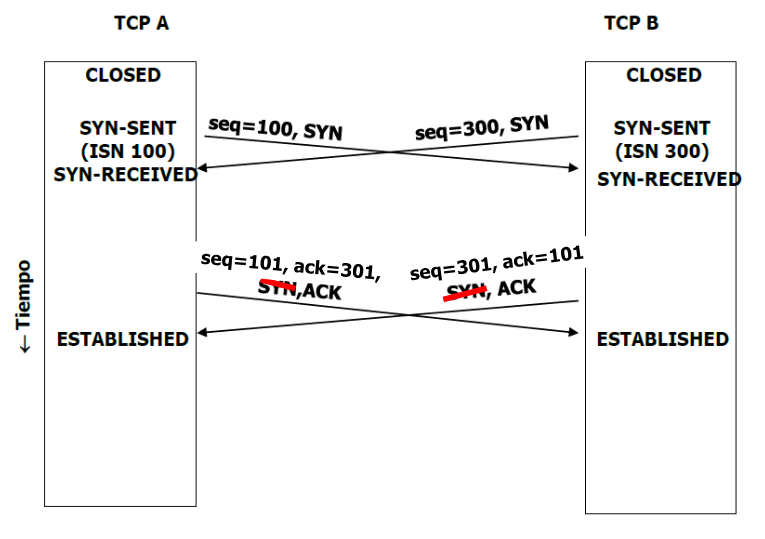
\includegraphics[width=0.7\textwidth]{images/control_conex_simultaneo.png}
    \caption{Proceso de Establecimiento de Conexión Simultánea en TCP}
    \label{fig:tcp_simultaneo}
\end{figure}

\subsubsection{Cierre de la Conexión TCP}

Se trata de la liberación de recursos y la finalización de la conexión. Para evitar bloqueos por pérdidas, una vez que comienza el proceso de cierre, se usan TimeOuts.

\begin{tcolorbox}[colback=red!5!white,colframe=red!75!black]
    MLS  = Maximum Segment Lifetime = 2 minutos
\end{tcolorbox}

\subsection{Control de Errores y Flujo}

El control de errores y de flujo son aspectos fundamentales del protocolo TCP para asegurar la entrega fiable y ordenada de los datos entre dos dispositivos. Estos mecanismos son esenciales para optimizar el rendimiento y garantizar que los datos se transmitan correctamente y sin pérdidas.\\\\
\textbf{Mejorar rendimiento $\rightarrow$ ventana deslizante.}  
Para mejorar el rendimiento y optimizar el uso del ancho de banda, TCP utiliza un mecanismo conocido como \textit{ventana deslizante} (sliding window). Este enfoque permite que el emisor envíe múltiples segmentos de datos sin esperar confirmaciones para cada uno, lo que mejora la eficiencia. La ventana deslizante controla cuántos datos puede enviar el emisor antes de que se necesite una confirmación. A medida que se reciben los segmentos, la ventana se desliza hacia adelante, permitiendo al emisor continuar enviando más datos..\\\\

\textbf{Control de errores: esquema ARQ con confirmaciones positivas y acumulativas.}  
TCP implementa un esquema de control de errores basado en ARQ (Automatic Repeat reQuest), que utiliza confirmaciones positivas y acumulativas. Esto significa que el receptor envía un mensaje de confirmación (ACK) para indicar que ha recibido correctamente los datos. Si el emisor no recibe esta confirmación en un tiempo determinado, retransmite el segmento de datos. Además, las confirmaciones son acumulativas, es decir, un solo ACK puede confirmar la recepción de múltiples segmentos de datos hasta un número determinado..\\\\

\textbf{Campos involucrados en el control de errores y flujo:}

- \textbf{Campo de secuencia:} Este campo contiene el número de secuencia del primer byte de datos en el segmento, lo que indica el offset (desplazamiento) en bytes dentro del mensaje. El número de secuencia es esencial para la reordenación de los segmentos en caso de que lleguen fuera de orden..\\\\
  
- \textbf{Campo de acuse de recibo (ACK):} Este campo contiene el número de byte esperado en el receptor. Cuando el receptor envía un ACK, está indicando el próximo byte que espera recibir. Este valor es crucial para el control de flujo, ya que ayuda al emisor a saber hasta qué punto los datos han sido recibidos correctamente... \\\\

- \textbf{Bit A (ACK) del campo de control:} El bit ACK en el campo de control se establece cuando el segmento es una confirmación de la recepción de datos. Si este bit está activado, significa que el receptor ha recibido correctamente los datos hasta el número de secuencia especificado en el campo de acuse de recibo..\\\\

- \textbf{Campo de comprobación (Checksum):} El campo de comprobación contiene un valor de verificación para asegurar la integridad del segmento de datos. Este valor se calcula aplicando un algoritmo de checksum sobre todo el segmento TCP, que incluye tanto los datos como la cabecera del segmento. Si el valor de checksum calculado en el receptor no coincide con el valor enviado en el segmento, se detecta un error y el segmento se descarta..\\\\

- \textbf{Uso de pseudo-cabecera TCP:} Para mejorar la fiabilidad del control de errores, TCP utiliza una pseudo-cabecera, que es un bloque de datos adicional utilizado en el cálculo del checksum. Esta pseudo-cabecera incluye la dirección IP de origen y destino, el protocolo (TCP) y la longitud de los datos, lo que ayuda a garantizar que los segmentos TCP se entreguen al destino correcto y no se corrompan durante la transmisión..\\\\

En conjunto, estos mecanismos de control de errores y de flujo permiten a TCP proporcionar una transmisión de datos fiable y eficiente, minimizando la posibilidad de errores y optimizando el uso del ancho de banda disponible..\\\\


\subsubsection{Pérdida de ACK y Timeout Prematuro con ACK Acumulativo}

En la imagen se muestran dos diagramas de secuencia que ilustran la comunicación entre dos hosts, Host A y Host B, en una red. La imagen está dividida en dos partes:\\

1. \textbf{Pérdida de ACK}: En esta parte del diagrama, Host A envía un paquete con el número de secuencia 92 y 8 bytes de datos a Host B. Host B recibe el paquete y envía un ACK con el número 100 de vuelta a Host A. Sin embargo, este ACK se pierde en la red (indicado por una X y la palabra pérdida). Debido a la pérdida del ACK, Host A no recibe la confirmación y, después de un tiempo de espera (timeout), retransmite el paquete con el número de secuencia 92 y 8 bytes de datos. Finalmente, Host B recibe el paquete retransmitido y envía nuevamente el ACK con el número 100.\\

2. \textbf{Timeout Prematuro y ACK Acumulativo}: En esta parte del diagrama, Host A envía un paquete con el número de secuencia 92 y 8 bytes de datos a Host B. Luego, Host A envía otro paquete con el número de secuencia 100 y 20 bytes de datos. Host B recibe ambos paquetes y envía un ACK con el número 100 y luego un ACK con el número 120 de vuelta a Host A. Sin embargo, debido a un timeout prematuro, Host A retransmite el paquete con el número de secuencia 92 y 8 bytes de datos antes de recibir el ACK acumulativo con el número 120. Finalmente, Host B recibe el paquete retransmitido y envía nuevamente el ACK con el número 120.\\

Este diagrama es relevante porque ilustra dos situaciones comunes en la comunicación de redes: la pérdida de ACK y el manejo de timeouts prematuros con ACK acumulativos. Estas situaciones son importantes para entender cómo los protocolos de comunicación, como TCP, manejan la retransmisión de paquetes y la confirmación de recepción para asegurar una comunicación confiable.\\

\begin{figure}[H]
    \centering
    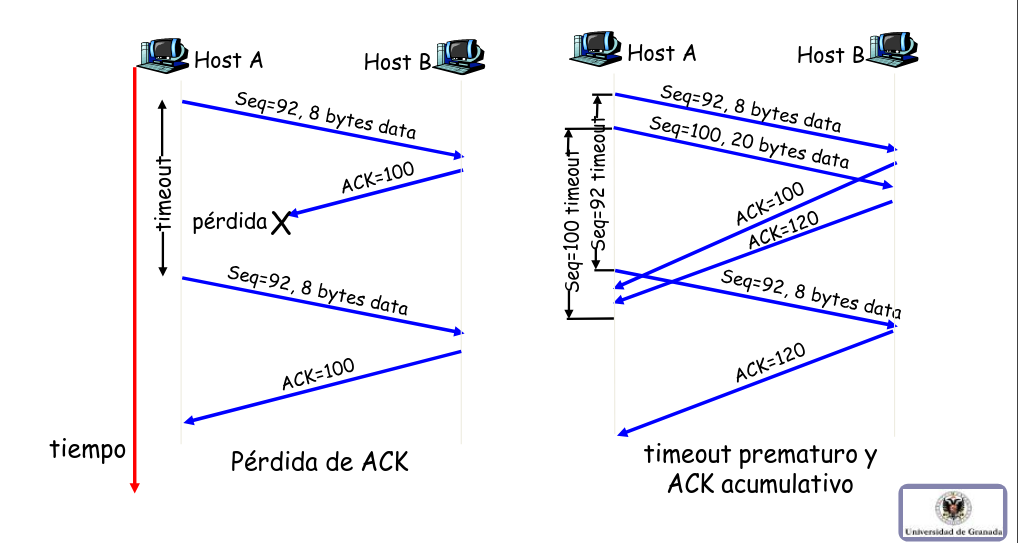
\includegraphics[width=0.7\textwidth]{images/control_errores.png}
    \caption{Pérdida de ACK y Timeout Prematuro con ACK Acumulativo}
    \label{fig:ack_timeout}
\end{figure}

\begin{table}[H]
    \centering
    \begin{tabular}{|p{8cm}|p{8cm}|}
    \hline
    \textbf{Evento} & \textbf{Acción del TCP receptor} \\ \hline
    Llegada ordenada de segmento, sin discontinuidad, todo lo anterior ya confirmado. & Retrasar ACK. Esperar recibir al siguiente segmento hasta 500 mseg. Si no llega, enviar ACK. \\ \hline
    Llegada ordenada de segmento, sin discontinuidad, hay pendiente un ACK retrasado. & Inmediatamente enviar un único ACK acumulativo. \\ \hline
    Llegada desordenada de segmento con \# de sec. mayor que el esperado, discontinuidad detectada. & Enviar un ACK duplicado, indicando el \# de sec. del siguiente byte esperado. \\ \hline
    Llegada de un segmento que completa una discontinuidad parcial o totalmente. & Confirmar ACK inmediatamente si el segmento comienza en el extremo inferior de la discontinuidad. \\ \hline
    \end{tabular}
    \caption{Eventos y acciones del receptor TCP}
\end{table}
    
\subsubsection{¿Cómo estimar los \textit{timeouts}?}

La estimación correcta de los \textit{timeouts} es crucial para el control de errores en las redes de computadoras. Un tiempo de espera (\textit{timeout}) demasiado pequeño puede llevar a \textit{timeouts} prematuros, mientras que uno demasiado grande puede resultar en una reacción lenta a la pérdida de segmentos. La mejor solución en situaciones cambiantes es adaptar los \textit{timeouts} de manera dinámica.

\textbf{RTTmedido}: tiempo desde la emisión de un segmento hasta la recepción del ACK.

La fórmula para calcular un nuevo valor de RTT (Round Trip Time) es la siguiente:

\[
\text{RTTnuevo} = \alpha \cdot \text{RTTviejo} + (1 - \alpha) \cdot \text{RTTmedido}, \quad \alpha \in [0,1]
\]

Donde:
\begin{itemize}
    \item \(\text{RTTnuevo}\): es el nuevo valor del RTT.
    \item \(\text{RTTviejo}\): es el valor anterior del RTT.
    \item \(\text{RTTmedido}\): es el RTT medido en la última transmisión.
    \item \(\alpha\): es un factor de ponderación entre 0 y 1.
\end{itemize}

Además, se debe calcular la desviación del RTT para tener en cuenta la variabilidad en los tiempos de transmisión. La fórmula es la siguiente:

\[
\text{Desviación}_{\text{nueva}} = (1 - x) \cdot \text{Desviación}_{\text{vieja}} + x \cdot \left| \text{RTTmedido} - \text{RTTnuevo} \right|
\]

Finalmente, el \textit{timeout} se calcula utilizando la siguiente fórmula:

\[
\text{Timeout} = \text{RTTnuevo} + 4 \cdot \text{Desviación}
\]

Esta estimación dinámica del \textit{timeout} asegura que los tiempos de espera se ajusten apropiadamente a las condiciones de la red, evitando tanto \textit{timeouts} prematuros como retrasos excesivos.

\subsubsection*{Problema con ACKs repetidos: ambigüedad en la interpretación}

La ambigüedad en la interpretación de ACKs repetidos puede complicar la estimación del RTT. La solución a este problema es utilizar el Algoritmo de Karn, que actualiza el RTT solo para aquellos segmentos que no presentan ambigüedad. Sin embargo, si es necesario repetir un segmento, se debe incrementar el \textit{timeout} de la siguiente manera:

\[
t_{\text{out}_{\text{nuevo}}} = \gamma \cdot t_{\text{out}_{\text{viejo}}}, \quad \gamma = 2
\]

Donde:
\begin{itemize}
    \item \( t_{\text{out}_{\text{nuevo}}} \): es el nuevo valor del \textit{timeout}.
    \item \( t_{\text{out}_{\text{viejo}}} \): es el valor anterior del \textit{timeout}.
    \item \( \gamma \): es un factor de multiplicación que generalmente se establece en 2.
\end{itemize}

Estas fórmulas y procedimientos permiten ajustar dinámicamente los tiempos de espera en las transmisiones TCP, mejorando la eficiencia y fiabilidad de las comunicaciones en redes de datos.

\subsubsection{Control de flujo}

Se trata del procedimiento en el que se controla lo que el emisor envía al receptor. Para ello, se utilizan ventanas de flujo, que son un mecanismo que permite al receptor controlar la cantidad de datos que el emisor puede enviar antes de recibir una confirmación. Es un esquema \textit{crediticio}, es decir, el receptor informa al emisor sobre los bytes autorizados a emitir sin esperar respuesta. 
\begin{equation}
    \text{Ventana útil emisor} = \text{Ventana ofertada receptor} - \text{bytes en tránsito}
\end{equation}

\begin{figure}[H]
    \centering
    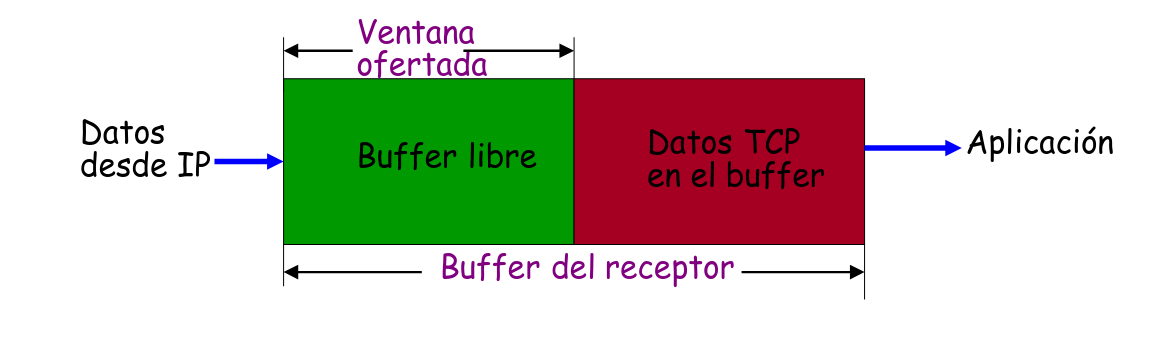
\includegraphics[width=0.7\textwidth]{images/control_flujo.png}
    \caption{Control de flujo en TCP}
\end{figure}

\subsubsection{Ejemplo Práctico: Control de Flujo en TCP}

\begin{figure}[H]
    \centering
    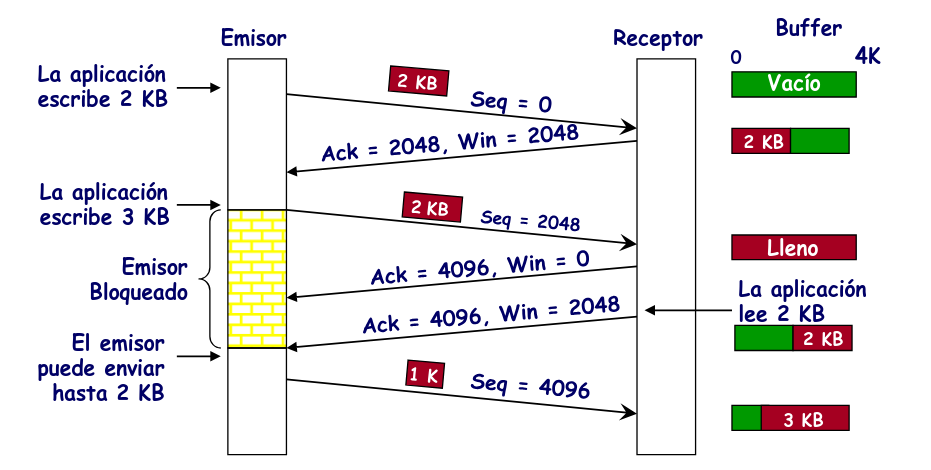
\includegraphics[width=0.7\textwidth]{images/control_flujo_proceso.png}
    \caption{Ejemplo práctico de control de flujo en TCP}
\end{figure}

\subsubsection*{Control de Flujo y Gestión de Buffer}

La imagen muestra un diagrama de comunicación entre un emisor y un receptor, con un enfoque en la gestión del buffer y el control de flujo en una red de transmisión de datos. A continuación, se detalla lo que sucede en cada paso:

1. \textbf{La aplicación escribe 2 KB}: El emisor envía 2 KB de datos al receptor con un número de secuencia (Seq) de 0.\\

2. \textbf{Ack = 2048, Win = 2048}: El receptor envía un acuse de recibo (Ack) indicando que ha recibido 2048 bytes y que su ventana de recepción (Win) es de 2048 bytes.\\

3. \textbf{La aplicación escribe 3 KB}: El emisor intenta enviar 3 KB de datos adicionales, pero solo puede enviar 2 KB debido a la ventana de recepción del receptor.\\

4. \textbf{Emisor Bloqueado}: El emisor está bloqueado porque no puede enviar más datos hasta que reciba un nuevo acuse de recibo del receptor.\\

5. \textbf{Ack = 4096, Win = 0}: El receptor envía un acuse de recibo indicando que ha recibido 4096 bytes, pero su ventana de recepción está llena (Win = 0).\\

6. \textbf{El emisor puede enviar hasta 2 KB}: El emisor recibe un nuevo acuse de recibo (Ack = 4096, Win = 2048) indicando que puede enviar hasta 2 KB más de datos.\\

7. \textbf{Seq = 4096}: El emisor envía 1 KB de datos adicionales con un número de secuencia de 4096.\\

El buffer del receptor se muestra en diferentes estados:
\begin{itemize}
    \item Inicialmente vacío.
    \item Luego con 2 KB de datos.
    \item Finalmente lleno con 4 KB de datos.
    \item Después de que la aplicación lee 2 KB, el buffer tiene 2 KB de datos y espacio para 2 KB más.
\end{itemize}


Este diagrama es relevante porque ilustra cómo se maneja el control de flujo y la gestión de buffers en una red de transmisión de datos, asegurando que los datos se envíen y reciban de manera eficiente sin perder información.\\


\subsubsection{Síndrome de la ventana tonta}

\begin{figure}[H]
    \centering
    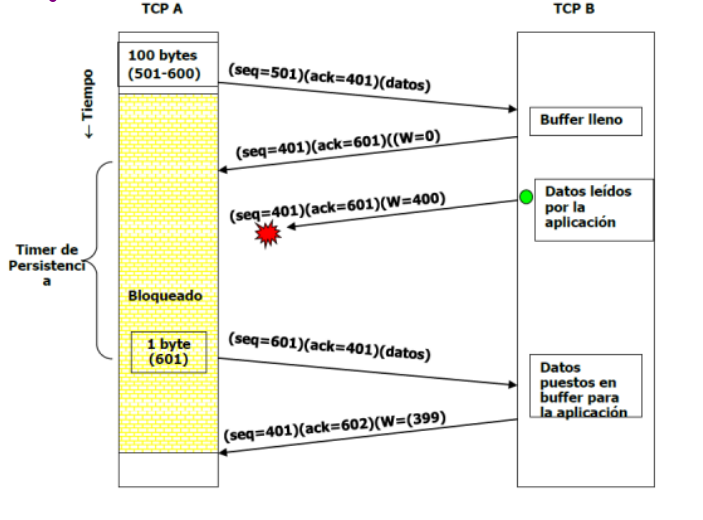
\includegraphics[width=0.7\textwidth]{images/ventana_tonta.png}
    \caption{Síndrome de la ventana tonta en TCP}
\end{figure}


\subsubsection*{Gestión del Flujo y del Tamaño de Ventana en TCP}

La imagen muestra una secuencia de eventos en una comunicación TCP (Transmission Control Protocol) entre dos entidades, TCP A y TCP B. Se ilustra el proceso de transmisión de datos, acuse de recibo (ACK) y gestión del tamaño de ventana (W). El diagrama está dividido en dos secciones principales: TCP A a la izquierda y TCP B a la derecha. En este caso en concreto se hace referencia al síndrome de la \textit{ventana tonta}, un problema que puede surgir en la gestión del flujo y del tamaño de ventana en TCP, que significa que el emisor envía datos a una velocidad más rápida que la q  ue el receptor puede procesar, lo que resulta en una baja eficiencia y un rendimiento subóptimo. Se puede solucionar con \textit{la ventana optimista}, que permite al emisor enviar datos a la máxima velocidad posible y ajustar la tasa de transmisión en función de la capacidad del receptor. Se pueden hace entregas no ordenadas y solicitar una entrega inmediata a la aplicación.\\

En TCP A:
\begin{itemize}
    \item \textbf{100 bytes (501-600)}: Inicialmente se envían 100 bytes con un número de secuencia (Seq) de 501 a 600.
    \item \textbf{(seq=501)(ack=401)(datos)}: TCP A envía datos con el número de secuencia 501 y espera un acuse de recibo para 401.
    \item \textbf{(seq=401)(ack=601)(W=0)}: TCP A recibe un acuse de recibo indicando que ha recibido 601 bytes, pero la ventana de recepción es 0, lo que significa que TCP A debe dejar de enviar datos temporalmente.
    \item \textbf{(seq=401)(ack=601)(W=400)}: TCP A envía un nuevo segmento con datos y recibe un acuse de recibo indicando que la ventana de recepción ha aumentado a 400 bytes.
    \item \textbf{(seq=601)(ack=401)(datos)}: TCP A envía datos adicionales con el número de secuencia 601.
    \item \textbf{(seq=401)(ack=602)(W=399)}: TCP A recibe un acuse de recibo indicando que ha recibido 602 bytes y que la ventana de recepción es de 399 bytes.
\end{itemize}

En TCP B:
\begin{itemize}
    \item \textbf{Buffer lleno}: El estado del buffer se indica mostrando que está lleno.
    \item \textbf{Datos leídos por la aplicación}: Los datos en el buffer son leídos por la aplicación.
    \item \textbf{Datos puestos en buffer para la aplicación}: Los datos son colocados en el buffer para ser leídos por la aplicación.
\end{itemize}

\subsection{Control de Gestión}

El control de congestión es un mecanismo fundamental en TCP para manejar la saturación en la red, descrito en la \textit{RFC 2001}. Este problema surge debido a la insuficiencia de recursos, como el ancho de banda de las líneas de transmisión, la capacidad de los buffers en los routers y los sistemas finales. La congestión puede degradar significativamente el rendimiento de la red si no se gestiona adecuadamente. Se trata de un problema debido a la insuficiencia de recursos (ancho de banda de las líneas como buffer en routers y sistemas finales.)\\

\textbf{Diferencias con el control de flujo.}  
Aunque puede parecer similar al control de flujo, el control de congestión aborda un problema diferente. Mientras que el control de flujo regula la cantidad de datos enviados para no sobrecargar al receptor, el control de congestión involucra tanto a la red como a los sistemas finales. Es una problemática que abarca todo el sistema de comunicación y no se limita a un enlace específico.\\

\textbf{Naturaleza adelante-atrás.}  
El control de congestión tiene una naturaleza de comunicación bidireccional (adelante-atrás), ya que los efectos de la congestión pueden propagarse en ambas direcciones del flujo de datos. Esto se manifiesta en:\\

- \textbf{Pérdidas de paquetes:} Los segmentos que no pueden ser almacenados en los buffers de los routers debido a la congestión son descartados.\\
- \textbf{Retrasos en las ACKs:} La congestión también provoca un incremento en los tiempos de transmisión de las confirmaciones (ACKs), lo que puede impactar el rendimiento del protocolo TCP.\\

\textbf{Solución: limitar de forma adaptable el tráfico generado.}  
La solución al problema de la congestión reside en que la fuente (el emisor) limite dinámicamente el tráfico generado, adaptándose a las condiciones de la red. Este enfoque incluye varios mecanismos clave:\\

- \textit{Congestion Window (cwnd):} TCP utiliza una ventana de congestión que controla cuántos datos pueden enviarse sin recibir ACKs. La ventana se ajusta dinámicamente según la retroalimentación de la red.\\

- \textit{Mecanismos de detección de congestión:} TCP responde a los indicadores de congestión, como pérdidas de paquetes o retrasos en las ACKs, disminuyendo la ventana de congestión para reducir el tráfico enviado.\\

- \textit{Recuperación adaptativa:} Después de detectar congestión, TCP incrementa gradualmente la ventana de congestión a medida que las condiciones de la red mejoran, utilizando técnicas como el \textit{Slow Start} y el \textit{Congestion Avoidance}.\\

En el emisor se utilizan dos ventanas y un umbral:
\begin{itemize}
    \item Bytes\_permitidos\_enviar = min(cwnd, rwnd\footnote{Ventana del receptor}).
    \item Ventana del receptor = se usa para el control de flujo de tamaño variable según el campo de ventana recibido.
    \item Inicialmente la ventana de congestión es de 1 MSS\footnote{Maximum Segment Size}.

\item Inicio Lento:
\begin{lstlisting}[style = customcpp]
    if (ventana de congestión < umbral, POR CADA ACK RECIBIDO){
        ventana de congestión ++ (crecimiento exponencial)
    }
\end{lstlisting}

\item Prevención de la congestión:

\begin{lstlisting}[style = customcpp]
    if (ventana de congestión > umbral, CADA VEZ QUE SE RECIBEN TODOS LOS ACKS PENDIENTES){
        ventana de congestión ++ (crecimiento lineal)
    }


    if (hay timeouts) {
        umbral = ventana de congestión / 2
        ventana de congestión = 1
    }
\end{lstlisting}

\section{Extensiones TCP}

Una de las definiciones de tcp es aquella en la que se expone que tiene múltiples \textit{sabores}, es decir, diferentes versiones que se adaptan a las necesidades de los usuarios. Estas versiones no afectan a la \textit{interoperabilidad} de los extremos. Se realizaron diversas modificaciones de manera que:
\begin{itemize}
    \item \textbf{Ventana escalada:} Esta opción se utiliza en los segmentos SYN de TCP para permitir una ventana de recepción más grande. Con la ventana escalada, el tamaño de la ventana puede aumentar hasta $2^{14} \times 2^{16} = 2^{30} = 1$ GB, lo que mejora significativamente el rendimiento en redes de alta capacidad y alta latencia.
    \item \textbf{Estimación de RTT:} La opción de sello de tiempo en TCP permite una estimación más precisa del RTT (Round Trip Time). Al incluir un sello de tiempo en todos los segmentos, TCP puede medir el tiempo exacto que tarda un segmento en ser reconocido, mejorando así la eficiencia del control de congestión y la retransmisión.
    \item \textbf{PAWS (Protection Against Wrapped Sequence Numbers):} Esta extensión utiliza sellos de tiempo para proteger contra la reutilización de números de secuencia. PAWS rechaza los segmentos duplicados que tienen sellos de tiempo más antiguos, asegurando que los datos se entreguen de manera ordenada y sin duplicaciones.
\end{itemize}


\end{itemize}
















%pag 17 de las diapos de mi tablet
%https://chatgpt.com/c/676fbc88-a0b4-8012-827b-90e2156977b7
%https://copilot.microsoft.com/chats/8CzyGkhcMFpGzg2Rtev1Q


\end{document}